\newpage
\begin{appendices}
\section{Evaluation of Existing Machine-learning based Name Generation Approaches for Generating Test Names}
\label[appendix]{sec:pilot-study}

Recent machine-learning based approaches (e.g.,~\cite{alon2018code2seq, alon2019code2vec}) performed significantly better on method and class name generation than previous approaches (e.g.,~\cite{allamanis2015suggesting, host2009debugging}).
%
However, it is unknown how well these machine-learning based approaches work in the context of generating names for unit tests.
%
To evaluate their performance for this task, we conducted a pilot study.

\subsection{Considered Name Generations Approaches}

As the state-of-the-art work on the topic of abstracting code to use it for name generation, \citeauthor{alon2018code2seq} proposed a series of novel approaches on representing code snippets as compositional paths or continuous distributed vectors~\cite{alon2018code2seq, alon2019code2vec}.
% TODO[fixed with both]: You need to be careful here.  Is there really an evaluation comparing all of these appraoches  Pretty sure no one compared them against Zhang?  If not you can't say that it outperforms.  Instead you can say something like ``it appears''  Or you can limit the claim to what is actually compared against which I think is other approaches for general name generation.
After an initial review of the results of their approaches, their generated test names outperformed some existing name generation and code abstraction techniques~\cite{host2009debugging,allamanis2015suggesting, allamanis2016convolutional,raychev2016probabilistic,bielik2016phog}.
%
It also appears to be better than other techniques that focused on providing better names\slash comments for methods, classes, and tests~\cite{ghafari2015automatically,sridhara2010towards,pradel2018deepbugs}.
%
The difference between the two approaches is that \texttt{Code2seq} encodes a code snippet to a set of compositional paths, and \texttt{Code2vec} encodes a code snippet to a fixed-length continuous vector.
%
Nonetheless, both of their approaches can make accurate prediction of Java method names.

\subsection{Considered Unit Tests}

\begin{table}[t]
\centering
\caption{Experimental Subjects.}
\begin{tabular}
{
  l
  l
  S[table-format=5.1]
  S[table-format=5.1]
}
\toprule
\multicolumn{1}{c}{\textbf{Project}} &
\multicolumn{1}{c}{\textbf{Version}} & 
\multicolumn{1}{c}{\textbf{LoC}} &
\multicolumn{1}{c}{\textbf{\# Tests}}
\\
\midrule
 Guice             & 9b371d3 &  183049  & 1280   \\
 Moshi             & dbed99d  &  22168  & 716   \\
 Picasso           & a087d26  &  11006  & 229  \\
 Fastjson          & e05f1f9  &  195511  & 4950   \\
 Guava             & 368c337  &  400801  & 13962  \\
 Mockito           & 22c82dc   &  59839 & 2145   \\
 Socket.io-client  & 661f1e7  &  9478  & 85  \\
 Scribejava        & ea42bc9  &  15184  & 110   \\
 ExoPlayer         & 79da521  &  172148  & 1510   \\
 Javapoet          & e9460b8  &  10755  & 302   \\
 Barbecue          & 44a8632  &  10760  & 170   \\
\bottomrule
\end{tabular}
\label{tab:subjectsForPilot}
\end{table}


To gather the tests we examined in our study, we started with the \num{11} Java projects \footnote{Same projects in the empirical study} shown in~\cref{tab:subjectsForPilot}.
%
In the table, the first column, \emph{Name}, shows the name of the project; the second column, \emph{Version}, shows the version of the project (either as a Git hash or version number); the fourth column, \emph{LoC}, shows the number of non-comment, non-blank lines of code as computed by SLOC count~\cite{nguyen2007sloc}; and the final column, \emph{\# Tests}, shows the number of unit tests in the project. In total, these \num{11} projects contain \num{25459} unit tests.
%
The first ten projects were randomly selected from the top \num{50} Java projects hosted on Github~\cite{top50projects}.
%
Because these projects encompass a variety of domains (e.g., JavaPoet is a library for generating Java programmatically and ExoPlayer is a media player for Android) and have many contributors (e.g., Moshi’s test suite contains contributions from \num{8} different people), their tests are more likely to be representative of tests in general which helps mitigate a potential threat to validity.
%
In addition, we also included Barbecue, a commonly used subject in the testing literature (e.g.,~\cite{zhang2015automatically, zhang2016towards, wu2020pattern}).
% TODO[added]: you could provide more details here.
\num{15400} tests were randomly selected from different test classes of the \num{11} projects to evaluate \texttt{Code2seq} and \texttt{Code2vec}.
%
The number of selected tests per project is roughly distributed by the quantity of tests in each project, which means we include more subjects from a project if it contains more tests.
%
We tried our best to randomly choose various tests from different types of test classes that are written by different developers (e.g., judging by their commits).


\subsection{Data and Discussion}

To generate the data necessary for investigating the quality of the generated names, we ran \texttt{Code2seq} and \texttt{Code2vec} on the set of \num{15400} tests.
%
Both \texttt{Code2seq} and \texttt{Code2vec} were run on a MacBook Pro (2.4GHz Intel i5 processor and 8GB RAM) with MacOS Mojave \footnote{Same machine in the empirical study}, Tensorflow 1.13.1 and Tensorflow 2.0.0, respectively.
% [Locally, changed to execution time only] Were you doing this locally or did you use the web interface?  This just seems really long.  Really just the execution time is what matters.
It took roughly \num{8} hours to both configure necessary environment and generating names for tests.


%TODO[replaced with better examples and description]: I want to see the bodies of these tests.  You want people to be able to see how the similarities in the bodies.
\Cref{fig:duplicate-names} shows an example of duplication the generated test names for both \texttt{Code2seq} and \texttt{Code2vec}.
%
For example in~\cref{fig:generated1}, it shows two tests from Barbecue and their generated names using \texttt{Code2seq}.
%
\texttt{test\-set\-non\-awt\-mode} is generated for both \texttt{test\-Non\-AWT\-Mode\-Always\-Returns\-Non\-AWT\-Environment} and \texttt{test\-Setting\-Non\-AWT\-Mode\-With\-No\-Resolution\-Uses\-Headless\-Environment\-Default\-Resolution}.


\begin{figure}[H]
\centering
\begin{subfigure}[b]{1.0\textwidth}
\centering
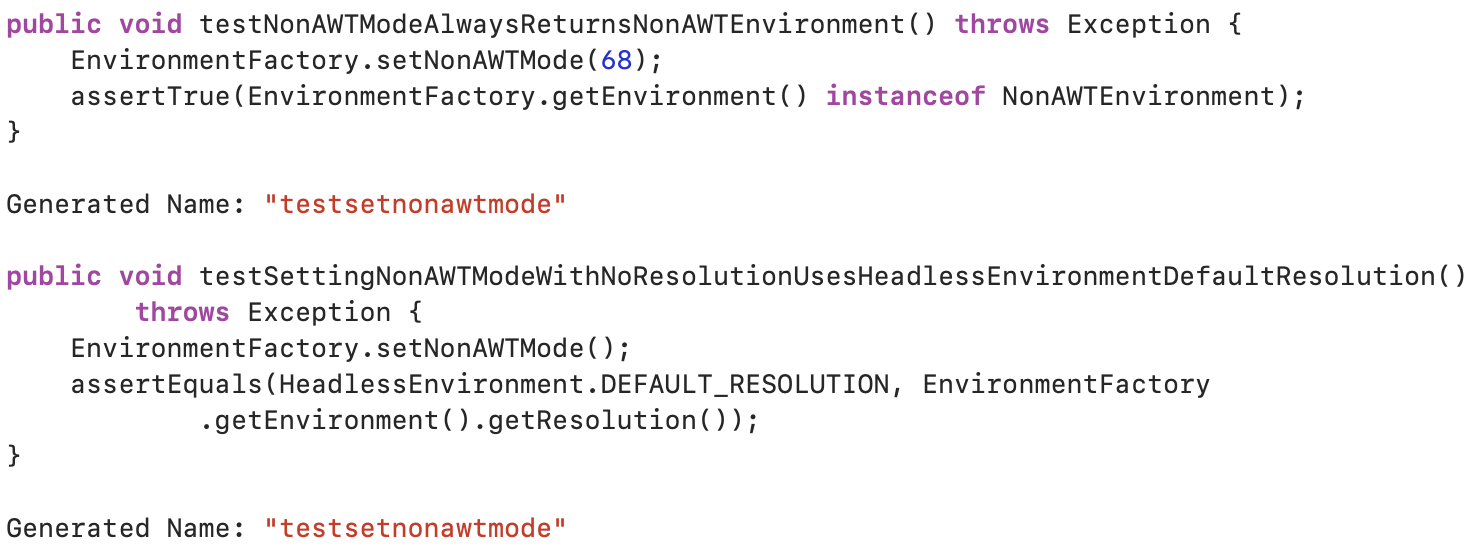
\includegraphics[scale=0.4]{figures/dup1.png}
\caption{Generated names by \texttt{Code2seq}.}
\label{fig:generated1}
\end{subfigure}\\
\vspace{0.2cm}
\begin{subfigure}[b]{1.0\textwidth}
\centering
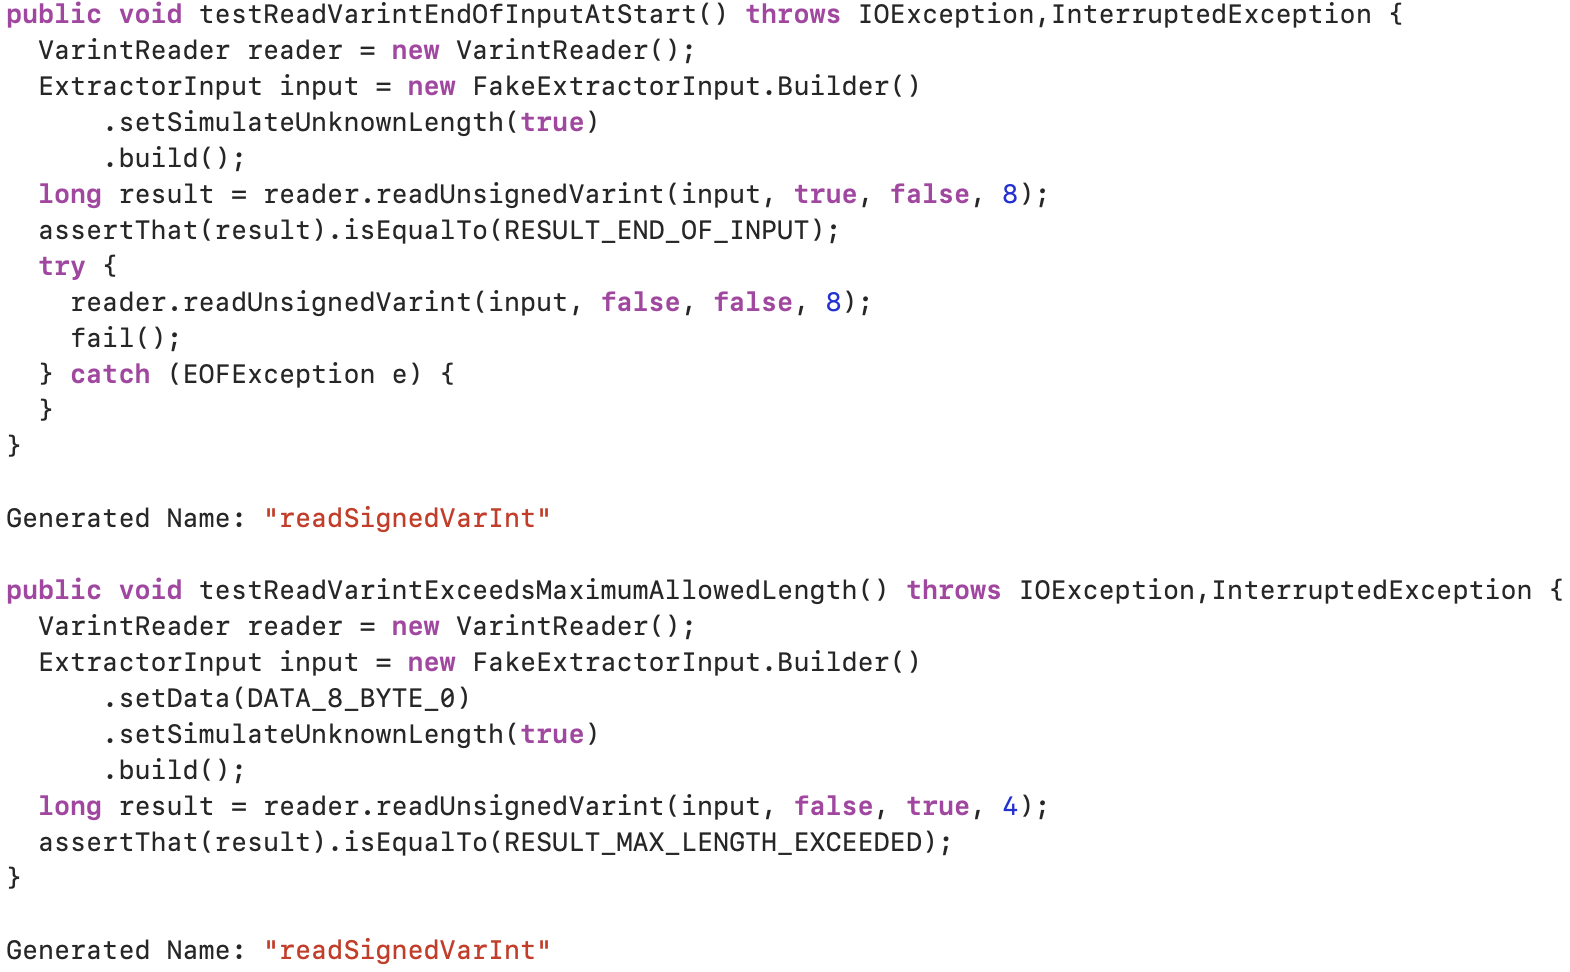
\includegraphics[scale=0.4]{figures/dup2.png}
\caption{Generated names by \texttt{Code2vec}.}
\label{fig:generated2}
\end{subfigure}
\caption{Example of generated names.}
\label{fig:duplicate-names}
\end{figure}


For another example in~\cref{fig:generated2}, it shows two test from ExoPlayer and their generated names by using \texttt{Code2vec}.
%
\texttt{read\-Signed\-Var\-Int} is generated for both \texttt{test\-Read\-Var\-int\-End\-Of\-Input\-At\-Start} and \texttt{test\-Read\-Var\-int\-Exceeds\-Maximum\-Allowed\-Length}.

Initially, our manual examination of the names was positive.
%
The names appeared to be descriptive at some level and were similar in format to existing test names.
%
However, we soon realized that both approaches frequently generated duplicate names for different tests in the same class.
%
Like in~\cref{fig:generated1}, \texttt{test\-Non\-AWT\-Mode\-Always\-Returns\-Non\-AWT\-Environment} and \texttt{test\-Setting\-Non\-AWT\-Mode\-With\-No\-Resolution\-Uses\-Headless\-Envir\-onment\-Default\-Resolution} are fundamentally different from each other, but \texttt{Code2seq} still generates the same name for both of them.
%
More importantly, their original test names are considered to be fully descriptive, and the descriptiveness in their original names comes from what make each test unique among its siblings.
%
For tests in~\cref{fig:generated1,fig:generated2}, the parameters in their assertions (i.e., actual or expected) make each test unique and are included in their original descriptive names.


\begin{table}[t]
\centering
\caption{Collected Data for \texttt{Code2seq} and \texttt{Code2vec}.}
\begin{tabular}
{
  l
  S[table-format=5.1]
  S[table-format=5.1]
}
 
\toprule
 & \multicolumn{2}{c}{\textbf{\# Duplicates}} \\
 \cmidrule(lr){2-3}
 
\multicolumn{1}{c}{\textbf{Project}} &
\multicolumn{1}{c}{\textbf{\texttt{Code2seq}}} &
\multicolumn{1}{c}{\textbf{\texttt{Code2vec}}}
\\
\midrule
 Guice             &  174   & 195   \\
 Moshi             &  80    & 98     \\
 Picasso           &  48    & 50     \\
 Fastjson          &  256   & 258   \\
 Guava             &  1152  & 1161  \\
 Mockito           &  254   & 328     \\
 Socket.io-client  &  15    & 15       \\
 Scribejava        &  17    & 22     \\
 ExoPlayer         &  240   & 257   \\
 Javapoet          &  46    & 52     \\
 Barbecue          &  30    & 18     \\
\bottomrule
\end{tabular}
\label{tab:ml-approach-data}
\end{table}


% TODO[fixed with new text]: I would like to see a table here.
% For each project show how many times a name is repeated in a test class.
% Then Update the discussion to match.
We collected and analyzed the generated test names from both \texttt{Code2seq} and \texttt{Code2vec}.
%
If many generated names are repeated at least once in its corresponding test class, it is necessary to develop a uniqueness-focused approach to solve the problem of duplication.
%
Since the complete data is is presented in a shared document~\cite{CodeResult}, so we show a crucial part of data from it in~\cref{tab:ml-approach-data}.
%
It shows tens or hundreds of duplicate names were generated for each project during their name generation process.
%
As a reminder, our set of subjects is just a subset of the tests in these projects.
%
In~\cref{tab:ml-approach-data}, each number represents how many times a generated name is repeated in a test class for each project, and each counted name is at least repeated once in its test class.
%
For example, the first rows shown \texttt{Code2seq} produced \num{174} duplicates, and \texttt{Code2vec} produced \num{195} duplicates, for ExoPlayer.
%
Both state-of-the-art approaches produced a significant number of duplicate names when performing their automated name generation on unit tests.
%
This result indicates there is a need to develop a uniqueness-focused approach that can extract unique attributes of tests to generate descriptive names.


\end{appendices}